\documentclass[a4paper]{article}

\usepackage{graphicx}
\usepackage{listings}
\usepackage{hyperref}

\lstset{
	tabsize=4,
	%basicstyle=\small \ttfamily,
	%basicstyle={\rmfamily},
	%basicstyle={\ttfamily},
	%numbers=left,
	numberstyle=\tiny,
	stepnumber=1,
	numbersep=5pt,
	frame=none,
}

\lstnewenvironment
	{matlab}
	{ 	\lstset{
			language=Matlab,
			%basicstyle=\small \ttfamily,
			frame=single,
			numbers=none
	}	}
	{ }

\lstnewenvironment
	{shell}
	{ 	\lstset{
			%language=Matlab,
			%basicstyle=\small \ttfamily,
			basicstyle={\ttfamily},
			frame=off,
			numbers=none
	}	}
	{ }

\newcommand{\nemo}{\texttt{NeMo}}
\newcommand{\code}[1]{\texttt{#1}}
\newcommand{\command}[1]{\texttt{#1}}
\newcommand{\file}[1]{\texttt{#1}}

% rst2latex leaves in title references
\newcommand{\titlereference}[1]{\textsl{#1}}

% rst2latex also sets this on inside the document
\newlength{\locallinewidth}

\input{title.tex}

\begin{document}

\maketitle

\section{Simulation}

\subsection{Neuron update}

During a single simulation cycle there are two main steps:
	current accumulation from incoming spikes,
	and update of the neuron state. 
Different orders of these two operations in otherwise identical simulators 
	will result in the firing times consistently differing by one,
	but with otherwise identical firing traces.

If the user provides external stimuli at specific times,
	the results may differ subtly depending on the exact time of insertion \emph{within} a cycle,
	in particular on how this insertion is ordered with respect to accumulation and state update.

\nemo\ performs each simulation step in the following order:

\begin{itemize}
	\item compute the accumulated current from incoming spikes;
	\item update the neuron state;
	\item determine if any neurons fired, which includes user stimuli in the form of forced firing;
	\item update the state of the fired neurons.
\end{itemize}

\subsection{Spike-timing dependant plasticity}
\label{stdp}

\nemo\ support spike-timing dependant plasticity,
	i.e.~synapses can change during simulation depending on the temporal relationship 
	between the firing of the pre- and post-synaptic neurons. 
To make use of STDP the user must first enable STDP globally by specifying an STDP function,
	and then enable plasticity for each desired synapse.
Currently only a single STDP function is applied to the whole network.

Synapses can be either potentiated or depressed.
With STDP enabled,
	the simulation accumulates a weight change, 
	which is the sum of potentiation and depression for each synapse. 
Potentiation always moves the synaptic weight away from zero,
	which for excitatory synapses is more positive,
	and for inhibitory synapses is more negative.
Depression always moves the synapses weight towards zero.
The accumulation of potentiation and depression statistics takes place every cycle,
	but the modification of the weight only takes place when explicitly requested.

Generally a synapse is potentiated if a spike arrives shortly before the
postsynaptic neuron fires. 
Conversely,
	if a spike arrives shortly after the postsynaptic firing the synapse is depressed. 
Also, the effect of either potentiation or depression generally weakens as the time difference, $dt$,
	between spike arrival and firing increases. 
Beyond certain values of $dt$ before or after the firing STDP has no effect. 
These limits for $dt$ specify the size of the \emph{STDP window}.

The user can specify the following aspects of the STDP function:

\begin{itemize}
	\item the size of the STDP window;
	\item what values of $dt$ cause potentiation and which cause depression;
	\item the strength of either potentiation or depression for each value of $dt$, i.e. the shape of the STDP function; and
	\item the maximum weight of any synapse.
\end{itemize}

Since the simulation is discrete-time,
	the STDP function can be sampled at the integer values for $dt$. 
For any value of $dt$, 
	a positive value of the function denotes potentiation, 
	while a negative value denotes depression.
The STDP function is described using two vectors: 
	one for spike arrivals \emph{before} the postsynaptic firing (pre-post pair), and
	one for spike arrivals \emph{after} the postsynaptic firing (post-pre pair).
The total length of these two vectors is the size of the STDP window.

In the common asymmetric scheme (Figure~\ref{fig:asymmetric}), 
	all spike arrivals (within the STDP window) before the postsynaptic firing cause potentation, 
	and all arrivals after the postsynaptic firing cause depression.
In other words, the whole prefire vector is postitive, while the whole postfire vector is negative. 
Note that the lengths of the two vectors need not be the same.

\begin{figure}[ht]
	\centering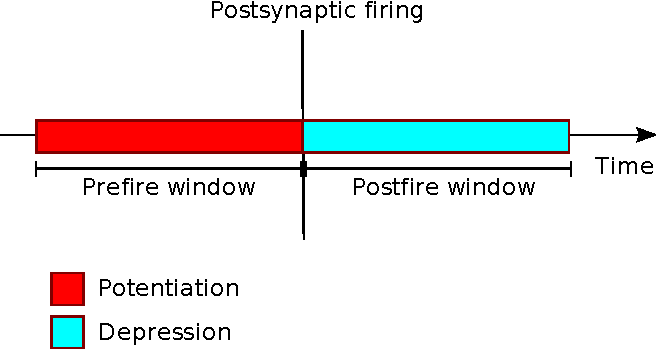
\includegraphics[width=.8\textwidth]{figures/stdp/asymmetric}
	\caption{Asymmetric STDP}
	\label{fig:asymmetric}
\end{figure}

A (more) \emph{symmetric} STDP function is shown in Figure~\ref{fig:symmetric}.  
Here both the prefire and postfire vectors contain both positive and negative values.

\begin{figure}
	\centering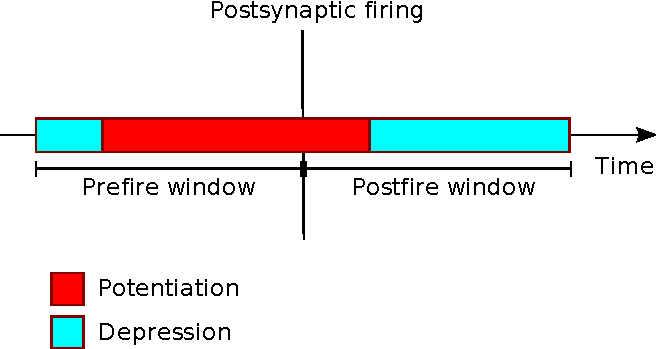
\includegraphics[width=.8\textwidth]{figures/stdp/symmetric}
	\caption{Symmetric STDP}
	\label{fig:symmetric}
\end{figure}

The lowest value for $dt$ on either side of the firing is 0. 
This value indicates that either the firing occurred as soon as possible after the spike
arrival, 
	or that the spike arrived as soon as possible after the firing. 
In the simulation one of these minima will be one cycle,
	rather than zero, but which it is depends on whether spike delivery takes place before or after firing during
the simulation of a single cycle. 
Both ways are reasonable choices, and the backends may use either.

Excitatory synapses are never potentiated beyond the user-specified maximum weight,
	and are never depressed below zero.
Likewise, inhibitory synapses are never potentiated beyond the  user-specified minimum weight,
	and are never depressed above zero.
Synapses can thus be deactivated, but never change from excitatory to inhibitory or vice versa.


%As a practical example, consider an asymmetric STDP scheme specified using the following functions for LTP and LTD:
%\[ stdp(dt) = \alpha e^{-dt / \tau} \]
%where $\alpha$ specifies a scaling and $\tau$ the size of either the potentiation or depression window. For LTP, let $\alpha = 1.0, \tau=20$, and for LTD let $alpha=0.8, \tau=20$. This STDP function is specified using two vectors like this:

%\section{Simulation backends}

\section{Running \nemo}

\nemo\ runs as a server process which serves client requests for constructing and running a network. 
\nemo\ thus requires an external client to control the simulation.
The interface uses a thrift protocol \cite{slee07thrift},
	which allows clients written in a number of languages including 
		Java,
		C++,
		Python,
		Perl, and 
		Haskell.
\nemo\ comes bundled with a Matlab interface (Section~\ref{api:matlab}).
Currently the only supported such frontend is Matlab.
Additional frontends are planned for Java and for Python (using a PyNN interface \cite{davison08pynn}). 

% TODO: add appendix with protocol

Figure~\ref{fig:rpc:basic} shows the basic setup.
The client communicates with the server using thrift over a TCP/IP transport.
The server uses one of several backends,
	such as one using the CPU, a GPU, or perhaps a cluster of computers.
The choice of backend is determined when the server is started,
	but does not affect the usage from the clients point of view.

\begin{figure}
	\includegraphics[width=\textwidth]{figures/rpc/basic}
	\caption{Communication between client and \nemo} 
	\label{fig:rpc:basic}
\end{figure}


\subsection{Pipelining}

Network communication can have significant overheads when running a simulation,
	especially if the client uses a very fine-grained control of the simulation,
	such as requesting data for every simulation step.
Pipelining can be used to reduce such overheads,
	by overlapping processing on the server with network traffic. 

In the non-pipelined setup shown in Figure~\ref{fig:rpc:basic},
	three main steps take place every time the client issues a simulation command: 
		the request is sent to the server,
		the server does some processing, and
		the reply is sent back to the client.
In a pipelined simulation (Figure~\ref{fig:rpc:pipelined}),
	these steps take place concurrently.
The request from the client is sent to and buffered on the client,
	while at the same time the server performs processing based on the previous
	request, 
	and sends the results based on the request from two steps ago. 
The data returned from the server for a single remote procedure call,
	is thus delayed by a few cycles.

\begin{figure}
	\includegraphics[width=\textwidth]{figures/rpc/pipelined_thrift}
	\caption{Pipelined communication between client and \nemo} 
	\label{fig:rpc:basic}
\end{figure}

\subsection{Matlab API}
\label{api:matlab}

\subsubsection{Installation}

The Matlab frontend is a collection of m-files and a pre-compiled binary, packed up in an archive.
To simply unpack to archive somewhere sensible and make sure the directory is on the Matlab path,
	which can be set in Matlab using \command{addpath <install-dir>}.
The \command{nemo} binary must be started externally prior to use.
This inconvenience will be removed in future versions.

\subsubsection{Reference implementation}

The Matlab distribution also contains a Matlab reference implementation.
This has exactly the same interface as the regular \nemo\ functions,
	but are implemented purely in Matlab.
The semantics of these functions replicate \nemo\ as far as possible.
Some divergence in results is bound to happen due to difference in floating point hardware etc.

There is one type of synapse structure which is not supported in the reference implementation.
Two neurons connected by two synapses (in the same direction), 
	with the same delay,
	can be represented in \nemo\ proper, but not in the reference implementation. 
Networks with such synapse pairs will have (more) divergent results on the two implementations if STDP is used.
A warning is issued if such duplicate synapses are found.
The script \file{mergeDuplicates.m}, bundled with the reference implementation)
	can be used to combine such synapses (by combining their weights).

\subsubsection{Usage}

The network is generated on the client side. 
The user should generate $n$-vectors 
	\code{a}, \code{b}, \code{c}, \code{d}, \code{u}, and \code{v} 
	that describe the neuron population. 
These vectors result in user-managed neuron indexing,
	which is 1-based as is usual in Matlab.
The connectivity is described using $n$-by-$m$ matrices specifying the 
	target neuron indices,
	synaptic weights,
	and delays.

A simple script which connects to a server,
	runs for 60 s with just a single firing stimulus,
	processing the returned firing data with the function \code{foo},
	could be written as follows:

% TODO: use matlab language file
%\begin{lstlisting}{language=Matlab}
\begin{matlab}
% ... code that generates the network
 
nemoConnect('axel01.doc.ic.ac.uk');
nemoSetNetwork(a, b, c, d, u, v,...
                targets, delays, weights);
nemoStartSimulation
for i=1:60
	fired = nemoRun(1000, [500 1]);
	foo(fired);
end
nemoStopSimulation;
nemoDisconnect;
\end{matlab}

or simpler, if 60 seconds worth of data can be processed (and buffered) at once:

\begin{matlab}
%  ... code that generates the network

nemoConnect('axel01.doc.ic.ac.uk');
nemoSetNetwork(a, b, c, d, u, v,...
                 targets, delays, weights);
nemoStartSimulation
fired = nemoRun(60000, [500 1]);
foo(fired);
nemoStopSimulation;
nemoDisconnect;
\end{matlab}

\subsubsection{Synaptic plasticity}

To make use of STDP the user must first specify the STDP function as described in Section~\ref{stdp}.
Additionally, the description of the connectivity matrix must now also specify which synapses are plastic. 
This is done via an extra argument to \code{nemoSetNetwork}.
By default all synapses are static.

To run for 1000ms applying STDP every 50ms, with all excitatory synapses being plastic, 
	do something like the following:

\begin{matlab}
% ... code that generates the network

nemoConnect('axel01.doc.ic.ac.uk');
prefire = 1.0 * exp(-(1:20)./20);
postfire = -0.8 * exp(-(1:20)./20);
nemoEnableSTDP(prefire, postfire, 30.0);
plastic = zeros(size(weights));
plastic(weights > 0) = 1;
nemoSetNetwork(a, b, c, d, u, v,...
                targets, delays, weights, plastic);
nemoStartSimulation
fired = nemoRun(50, [1 1]);
for i=50:50:1000
	nemoApplySTDP(1.0);
	fired = nemoRun(50, []);
	foo(fired);
end
nemoStopSimulation;
nemoDisconnect;
\end{matlab}

The vectors \code{prefire} and \code{postfire} specify the STDP function in the prefire and postfire parts of the STDP window. 
The length of these vectors specify the size of the STDP window.
See Section~\ref{stdp} for more information.


\subsubsection{Troubleshooting}

\paragraph{Calling MEX function results in warning regarding compiler version}

This problem is described in some detail here: 
%\hyperref{http://www.mathworks.com/support/solutions/data/1-2H64MF.html}.
One workaround mentioned there is to set the \code{LD\_PRELOAD} environment variable
before starting Matlab. For \command{bash}:

\begin{shell}
export LD_PRELOAD=/lib/libgcc_s.so.1
\end{shell}
and for \command{csh}:
\begin{shell}
setenv LD_PRELOAD /lib/libgcc_s.so.1
\end{shell}

\paragraph{Matlab fails with \texttt{Invalid MEX-file}, \texttt{libnemoclient.so: cannot open shared object file: No such file or directory.}}

Check that the directory containing the library files are in the system library
path. E.g. using \command{bash}:

\begin{shell}
export LD_LIBRARY_PATH=/path/to/nemo
\end{shell}


\subsubsection{Alphabetical function reference}

The following reference documentation is also available from inside matlab by calling \texttt{help <function>}.

\input{matlab}

\bibliographystyle{abbrv}
\bibliography{manual}

\end{document}
